% !TeX spellcheck = sk_SK-Slovak
% !TeX root = statnicaEKT.tex
%%======= Balicky ======%%
%\documentclass[12pt,a4paper]{sablonaMVA}
%\usepackage{graphicx}
%\usepackage{multirow}
%\usepackage{multicol}
%\usepackage{array}
%\usepackage{lipsum}
%\usepackage{blindtext}
%\usepackage{nicematrix}
%\usepackage{wrapfig}
%\usepackage{caption}
%\usepackage{subcaption}
%\usepackage{amsmath}
%\usepackage{float}
%\usepackage{amssymb}
%\usepackage{hyperref}
%\usepackage{siunitx}
%\usepackage{relsize}
%\sisetup{detect-all}
%\usepackage[english,slovak]{babel}  \usepackage[T1]{fontenc}
%\usepackage{booktabs}
%\usepackage{makecell}
%\usepackage{numerica}
%\usepackage[normalem]{ulem}
%\usepackage{tikz}
%\usepackage{etoolbox}
%\usepackage{esint}
%\usepackage{enumitem}
%\preto\tabular{\shorthandoff{-}}

%====== Vyplňte údaje ======
%\documentclass[a4paper,12pt]{article}
%\usepackage[a4paper,margin=2cm]{geometry}
%\usepackage[most]{tcolorbox}
%\usepackage{xcolor}
%\usepackage{ragged2e}
%
%\newcommand{\uloosdot}[1]{%
%	\tikz[baseline=(todotted.base)]{
%		\node[inner sep=1pt,outer sep=0pt] (todotted) {#1};
%		\draw[loosely dotted] (todotted.south west) -- (todotted.south east);
%	}%
%}%

%\begin{document}
% ===================== HLAVIČKA DOKUMENTU =====================
% Definícia farieb podľa predlohy
%\definecolor{nadpisblue}{RGB}{18,32,115}
%\definecolor{boxgray}{RGB}{230,230,230}
%\definecolor{boxborder}{RGB}{90,110,180}

% Pravý horný roh
%\begin{flushright}
%	\small
%	\textbf{BPC-ANT, Antény a vedení}\\
%	Vypracované otázky k SZZ od družiny vajčakov  
%\end{flushright}
%\raggedright
%%\vspace*{-10mm}
\graphicspath{{./Obrazky/}}
\part{BPC-ANT - Antény a Vedení}
{\huge
Otázky:}
\begin{enumerate}
	\item Šíření elektromagnetických vln (intenzita pole, vlnová rovnice, délka vlny, fázová rychlost, vlnové číslo, vlnová impedance, Poyntingův vektor). Rovinná a kulová vlna.
	\item Přenosová vedení (telegrafní rovnice, konstanta šíření, charakteristická impedance, transformace impedance vedením, Smithův diagram, impedanční přizpůsobení). Koaxiální vedení.
	\item Antény (elementární zářič, technický výpočet záření anténních soustav, směrová charakteristika, směrovost, zisk, polarizace, vstupní impedance, ekvivalentní obvod). Dipólové a flíčkové antény.
\end{enumerate}

\chapter{Šíření elektromagnetických vln. Rovinná a kulová vlna.}

\subsection{Intenzita poľa}
% Elektromagnetická vlna predstavuje spôsob prenos elektromagnetickej energie priestorom\\
% -- je založené na prelievaní energie elektrického poľa do magnetického poľa a naopak\\

%\vspace{-1mm}
\noindent
\begin{minipage}[t]{0.48\textwidth}
	{\centering
	\textbf{Intenzita mag. poľa}
	\begin{equation}
		\oint_{l} \mathbf{H}\cdot d\mathbf{l} = i + \frac{d\psi}{dt}
		\label{Amper_zakon}
	\end{equation}}
	\raggedright
	\underline{Ampérov zákon} popisuje prelievanie energie elektrického poľa do magnetického poľa.\par
	\medskip
	V prípade, že tečie tenkým drôtom vodivý prúd $i$ a posuvný prúd $d\psi/dt$, vzniknú okolo vodiča prstencové siločiary magnetického poľa.\\
	\medskip
	$\mathbf{H}$ [A/m] -- intenzita mag. poľa\\ 
	d$\mathbf{l}$ -- elementárny úsek
	
%	$\mathbf{H}$ [A/m] - intenzita magnetického poľa,\\ d$\mathbf{l}$ - elementárny úsek\\
%	Ak tečie tenkým drôtom vodivý prúd $i$ a posuvný prúd $d\psi/dt$, vzniknú okolo vodiča prstencové siločiary magnetického poľa
%	}
%	\begin{itemize}[label = --]
%	%\vspace{-2mm}
%	\item popisuje prelievanie energie elektrického poľa do magnetického poľa
%	\item ak tečie tenkým drôtom vodivý prúd $i$ a posuvný prúd $d\psi/dt$, vzniknú okolo vodiča prstencové siločiary magnetického poľa
%	\item intenzita magnetického poľa $\mathbf{H}$ má jednotku [A/m] a d$\mathbf{l}$ je elementárny úsek
%	\end{itemize}
\end{minipage}
\hfill
\begin{minipage}[t]{0.48\textwidth}
	\centering
	\textbf{Intenzita el. poľa}
	\begin{equation}
		\oint_{l} \mathbf{E}\cdot d\mathbf{l} = -\frac{d\Phi}{dt}
		\label{Faradayov_zakon}
	\end{equation}
	\raggedright
	\underline{Faradayov zákon} popisuje prelievanie energie magnetického poľa do elektrického poľa.\\
	\medskip
	Časovou zmenu magnetického indukčného toku $d\phi/dt$ je na svorkách vodivej slučky indukované napätie.\\
	\medskip
	$\mathbf{E}$ [V/m] -- intenzita el. poľa\\ 
	d$\mathbf{l}$ -- elementárny úsek		
\end{minipage}
%\vspace{5mm}

\subsection{Vlnová rovnica}

\begin{minipage}[t]{0.48\textwidth}
	\begin{equation}
		\nabla^2\mathbf{H} + k^2\mathbf{H} = \mathbf{0}
	\end{equation}
\end{minipage}
	\hfill
\begin{minipage}[t]{0.48\textwidth}
	\begin{equation}
		\nabla^2\mathbf{E} + k^2\mathbf{E} = \mathbf{0}
	\end{equation}
\end{minipage}\\
\bigskip
Vlnová rovnica popisuje šírenie elektromagnetickej vlny priestorom. Vyplýva z Maxwellových rovníc -- elektrické pole vytvára magnetické pole a naopak. Jej riešením je možné zistiť intenzitu poľa kdekoľvek v priestore.

Všeobecným riešením sú dve vlny - priama a spätná
\begin{equation}
	E_x = A exp(-jkz) + B exp(+jkz)
\end{equation}
Člen $A\exp(-jkz)$ predstavuje vlnu postupujúcu v smere $+z$, člen $B\exp(+jkz)$ vlnu spätnú (napr. odraz od prekážky).

\subsection{Dĺžka vlny}
Vlnová dĺžka $\lambda$ [m] je definovaná ako najkratšia vzdialenosť dvoch miest, v ktorých ma vlna rovnakú fázu.

\begin{equation}
	\lambda = c T = \frac{c}{f}
\end{equation}

Ak vlna smeruje pod uhlom $\alpha$ vôči osi $x$, vlnová dĺžka meraná v smere osi y je väčšia:
\begin{equation}
	\lambda_y = \frac{\lambda}{\sin(\alpha)}
\end{equation}

V hustejšom prostredí ($\varepsilon_r > 1$ alebo $\mu_r > 1$) je vlnová dĺžka kratšia než vo vákuu:
%Vlnová dĺžka bude v hustejšom prostredí kratšia:
\begin{equation}
	\lambda = \frac{c}{\sqrt{\mu_r \varepsilon_r}} \cdot T = \frac{\lambda_0}{\sqrt{\mu_r \varepsilon_r}}
\end{equation}

\subsection{Fázová rýchlosť}

V hustejšom prostredí ($\varepsilon_r > 1$ alebo $\mu_r > 1$) je rýchlosť šírenia je vôči vákuu nižšia:

\begin{equation}
	v_f = \frac{c}{\sqrt{\mu_r \varepsilon_r}}
\end{equation}

Ak vlna smeruje pod uhlom $\alpha$ vôči ose, vlnová dĺžka meraná v smere osi y je väčšia:
\begin{equation}
	v_{fy} = \frac{v_f}{\sin(\alpha)}
\end{equation}


\subsection{Vlnové číslo}

Vlnové číslo $k$ je komplexná konštanta šírenia, ktorá nesie informáciu o tom, ako sa vlna mení v priestore:
%\vspace{-1mm}
\begin{equation}
	k = k' - jk''
\end{equation}

kde:\\
-- $k'$ [rad/m] -- merná fáza: o koľko radiánov sa zmení fáza na 1 meter dráhy\\
-- $k''$ [1/m] -- merný útlm: ako rýchlo klesá amplitúda vlny (závisí od vodivosti prostredia $\xi$)\\
\medskip
V bezstratovom prostredí ($\xi$ = 0) je $k'' = 0$ -- vlna sa šíri bez útlmu a $k$ je čisto reálne:

\begin{equation}
	k' = \omega \frac{\sqrt{\mu_r \varepsilon_r}}{c}
\end{equation}

\subsection{Vlnová impedancia}

Vlnová impedancia prostredia $Z_0$ [$\Omega$] je konštanta úmernosti medzi intenzitou elektrického a magnetického poľa:
\begin{equation}
	Z_0 = \sqrt{\frac{j\omega\mu}{\gamma + j\omega\varepsilon}}
\end{equation}

\subsection{Pointingov vektor}

Poyntingov vektor $\Pi$ vyjadruje plošnú hustotu výkonu neseného elektromagnetickou vlnou. Jeho smer je totožný so smerom šírenia vlny:
\begin{equation}
	\Pi = \mathbf{E} \times \mathbf{H^\ast}
\end{equation}
Vo vzťahu značí symbol $\times$ vektorový súčin a $\ast$ komplexná združenosť zložiek vektoru $\mathbf{H^2}$

\subsection{Rovinná vlna}

	 Vlnoplocha leží v rovine $xy$ a vlna sa šíri v smere osi z. Amplitúda elektrickej a magnetickej intenzity je na vlnoploche konštantná (vlna je uniformná). Vektory $E$ a $H$ sú kolmé na smer šírenia aj navzájom — vlna je priečne elektromagnetická (TEM), teda nemá pozdĺžne (longitudinálne) zložky. V bezstratovom prostredí amplitúda v smere šírenia neklesá, mení sa len fáza. Zdrojom rovinnej vlny je v praxi vzdialený bodový žiarič — zakrivenie vlnoplôch je tak malé, že ich považujeme za roviny.
	 
	\begin{figure}[H]
	%\vspace{-2mm}
	\makebox[\textwidth]{%
		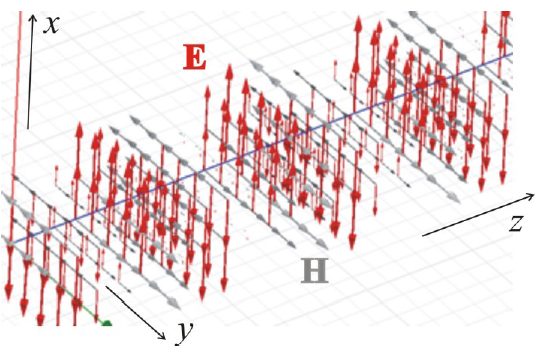
\includegraphics[scale=0.6]{ANT/rovinna_vlna.png}}
	\caption{Šírenie rovinnej vlny vo voľnom priestore}
	\end{figure}

\subsection{Guľová vlna}

Zdrojom je všesmerový (izotropný) bodový žiarič. Vlnoplochy sú sústredené guľové povrchy so stredom v zdrojovom žiariči. Amplitúda klesá nepriamo úmerne s vzdialenosťou $r$ od zdroja, pretože výkon prechádzajúci ľubovoľnou guľovou plochou musí byť v bezstrátovom prostredí konštantný -- z toho vyplýva $E\approx 1/r$. Efektívna hodnota elektrickej intenzity vo vzdialenosti $r$ od zdroja so vyžarovaným výkonom $P_\Sigma$ je:

\begin{equation}
	E_{ef} = \frac{\sqrt{30 P_\Sigma}}{r} \cdot \sqrt[4]{\frac{\mu_r}{\epsilon_r}}
\end{equation}

Skutočné zdroje nie sú izotropné, preto sa zavádza činiteľ smerovosti $D(\varphi, \vartheta)$, ktorý je väčší ako 1 v smeroch, do ktorých zdroj žiarenie sústreďuje, a menší ako 1 tam, kde je žiarenie potlačené.

\begin{equation}
	E_{ef} = \frac{\sqrt{30 P_\Sigma D(\varphi, \vartheta)}}{r} \cdot \sqrt[4]{\frac{\mu_r}{\epsilon_r}}
\end{equation}

\chapter{Přenosová vedení, Koaxiální vedení.}

\subsection{Koaxiálne vedenie}
Koaxiálny kábel pozostáva z vysoko elektricky vodivého vnútorného a vonkajšieho vodiča, medzi ktorými je homogénna dielektrická výplň s permitivitou $\varepsilon_r$ a permeabilitou $\mu_r$. \par
V koaxiálnom kabelu je elektromagnetické pole ''uväznené'' v dielektriku medzi vonkajším vodičom a vnútorným vodičom. Vlna sa šíri v smere osy vedenia.\par
\bigskip
Na obr. \ref{fig:koax_pole}  sú zobrazené siločiary elektrického a magnetického poľa v priečnom priereze vedenia.
Vlna sa šíri v smere osi koaxiálneho vedenia ako TEM vlna — siločiary elektrického poľa sú radiálne, siločiary magnetického poľa tvoria sústredné kružnice, oba vektory sú kolmé na smer šírenia. Súčasne sú siločiary magnetického poľa kolmé k siločiaram elektrického poľa.

	\begin{figure}[H]
	%\vspace{-2mm}
	\makebox[\textwidth]{%
		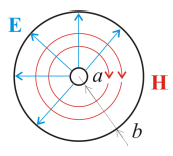
\includegraphics[scale=0.75]{ANT/koax_pole.png}}
	\caption{Rozloženie poľa v priečnom priereze koaxiálneho vedenia}
	\label{fig:koax_pole}
\end{figure}

Napätie medzi vodičmi vedenia:
\begin{equation}
	U = E(r) r \ln \left( \frac{b}{a} \right)
\end{equation}

Prúd pretekajúci vodičmi vedenia:
\begin{equation}
	I = 2 \pi r H
\end{equation}

Charakteristická impedancia koaxiálneho vedenia je:
\begin{equation}
	Z_v = \frac{1}{2\pi} \sqrt{\frac{\mu}{\varepsilon}} ln \frac{b}{a}
\end{equation}

\subsection{Telegrafní rovnice}

Telegrafné rovnice popisujú, ako sa napätie a prúd menia pozdĺž prenosového vedenia. Pre analýzu sú zavedené:
\begin{itemize}[label = --]
\item $R_1$ [$\Omega$/m] - odpor
\item $L_1$ [L/m] - indukčnosť
\item $C_1$ [F/m] - kapacita
\item $G_1$ [S/m] - vodivosť
\end{itemize}

\begin{figure}[H]
	%\vspace{-2mm}
	\makebox[\textwidth]{%
		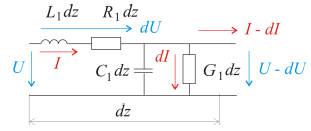
\includegraphics[scale=0.7]{ANT/nahradna_schema_vedenia.png}}
	\captionsetup{justification=centering}
	\caption{Náhradne schéma dvojvodičového vedenia}
	\label{fig:nahradna_schema_vedenia}
\end{figure}

\textbf{Telegrafné rovnice:}\\
\textbf{1. rovnica} hovorí, že napätie na vedení klesá v smere šírenia vplyvom pozdĺžnej impedancie $Z_1$
(odpor a indukčnosť vodiča). \\
\textbf{2. rovnica} hovorí, že prúd klesá vplyvom priečnej admitancie $Y_1$ (kapacita a vodivosť dielektrika medzi vodičmi). 

\begin{minipage}[t]{0.48\textwidth}
	\begin{equation}
		d^2U/dz^2 = UZ_1Y_1
	\end{equation}
\end{minipage}%
\begin{minipage}[t]{0.48\textwidth}
	\begin{equation}
		d^2I/dz^2 = IZ_1Y_1
	\end{equation}
\end{minipage}
\bigskip

Ich kombináciou dostaneme rovnice, ktoré majú rovnakú štruktúru ako vlnová rovnica — riešením sú teda dve vlny, priama šíriaca sa od zdroja k záťaži a spätná šíriaca sa od záťaže späť k zdroju.
\subsection{Konštanta šírenia}

Konštanta šírenia $\gamma$ určuje, ako sa vlna napätia a prúdu mení pozdĺž vedenia. 
\begin{equation}
	\gamma = \beta + j\alpha
\end{equation}
kde:\\ $\beta$ [m$^{-1}$] je merný útlm, ktorý určuje ako rýchlo amplitúda vlny klesá v smere šírenia vplyvom strát v odpore vodiča a vodivosti dielektrika, \\$\alpha$ [rad/m] je merná fáza, ktorá určuje ako rýchlo sa mení fáza vlny pozdĺž vedenia, $\alpha = 2\pi / \lambda_v$.\\
\bigskip
Všeobecné riešenie telegrafných rovníc má tvar:
\begin{equation}
	U(z) = A \exp (- \gamma z) + B \exp(+ \gamma z)
\end{equation}

\begin{equation}
	I(z) = \frac{1}{Z_V} [A \exp (- \gamma z) - B \exp(+ \gamma z)]
\end{equation}

kde $\gamma$ je konštanta šírenia (súčiniteľ prenosu):
\begin{equation}
	\gamma = \sqrt{(R_1 + j\omega L_1)(G_1 + j \omega C_1)}
\end{equation}
Člen $\exp (-\gamma z) $ predstavuje \textbf{priamu} vlnu šíriacu sa od zdroja k záťaži, člen $\exp (+\gamma z) $ predstavuje \textbf{spätnú} (odrazenú) vlnu šíriacu sa od záťaže späť k zdroju.

\subsection{Charakteristická impedancia}
Charakteristická impedancia vedenia $Z_v$ je pomer napätia a prúdu priamej (alebo spätnej) vlny:
\begin{equation}
	Z_v = \sqrt{\frac{R_1 + j \omega L_1}{G_1 + j \omega C_1}}
\end{equation}

Pomer celkového napätia a celkového prúdu sa charakteristickej impedancii rovná len vtedy, ak na vedení nie je spätná vlna -- vedenie je prispôsobené ($Z_k = Z_v$)

\subsection{Činiteľ odrazu a stojaté vlnenie}

Ak je vedenie zakončené záťažou $Z_k \neq Z_V$, odráža sa časť energie 
priamej vlny späť k zdroju ako vlna spätná. Pomer napätia spätnej 
a priamej vlny nazývame \textbf{činiteľom odrazu}:

\begin{equation}
	\rho(\zeta) = \frac{U^Z(\zeta)}{U^P(\zeta)} = -\frac{I^Z(\zeta)}{I^P(\zeta)}
\end{equation}

%Činiteľ odrazu môžeme vypočítať aj z impedancie vedenia v danom mieste 
%$\zeta$ a charakteristickej impedancie $Z_V$:
%
%\begin{equation}
%	\rho(\zeta) = \frac{Z(\zeta) - Z_V}{Z(\zeta) + Z_V}
%\end{equation}
%
%So vzdialenosťou od konca vedenia sa mení ako 
%$\rho(\zeta) = \rho(0)\exp(-2\gamma\zeta)$ — jeho modul pri stratovom 
%vedení klesá smerom k zdroju a fáza sa otáča. Je-li vedenie zakončené 
%charakteristickou impedanciou $Z_k = Z_V$, je $\rho = 0$ a všetka 
%energia priamej vlny sa spotrebuje v záťaži.

\subsection{Vznik stojatého vlnenia}

Celkové napätie a prúd na vedení sú superpozíciou priamej a spätnej vlny:

\begin{equation}
	U(\zeta) = U^P(0)\exp(+\gamma\zeta) + U^Z(0)\exp(-\gamma\zeta)
\end{equation}
\begin{equation}
	I(\zeta) = I^P(0)\exp(+\gamma\zeta) - I^Z(0)\exp(-\gamma\zeta)
\end{equation}

\newpage
Priama a spätná vlna sa stretávajú a ich súčtom vzniká \textbf{stojaté 
	vlnenie} — vlna, ktorá sa nešíri, ale kmitá na mieste. Rozlišujeme 
dve charakteristické miesta:

\begin{itemize}
	\item \textbf{Kmitňa} — miesto, kde sa priama a spätná vlna 
	stretávajú vo fáze; amplitúda je maximálna 
	$U_{max} = U^P + U^Z$.
	\item \textbf{Uzol} — miesto, kde sú priama a spätná vlna 
	v protifáze; amplitúda je minimálna 
	$U_{min} = U^P - U^Z$.
\end{itemize}

V miestach uzlov napätia sa nachádzajú kmitne prúdu a naopak. Vyplýva to z toho, že napätie 
je dané súčtom priamej a spätnej vlny, zatiaľ čo prúd je ich rozdielom.

\subsection{Pomer stojatých vĺn}

Stojaté vlnenie sa kvantifikuje \textbf{pomerom stojatých vĺn (PSV)} 
— pomerom amplitúdy napätia v kmitni k amplitúde v uzle:

\begin{equation}
	PSV = \frac{U_{max}}{U_{min}} = \frac{I_{max}}{I_{min}} 
	= \frac{1 + |\rho|}{1 - |\rho|}
\end{equation}

Rozlišujeme dva krajné prípady:

\begin{itemize}
	\item \textbf{Postupná vlna} ($PSV = 1$, $\rho = 0$) — šíri sa 
	len priama vlna, záťaž spotrebuje všetku energiu. Nastáva 
	pri $Z_k = Z_V$.
	\item \textbf{Čiste stojatá vlna} ($PSV \to \infty$, $|\rho| = 1$) 
	— energia sa neprenáša, iba kmitá medzi zdrojom a záťažou. 
	Nastáva pri zakončení nakrátko ($Z_k = 0$) alebo 
	naprázdno ($Z_k \to \infty$).
\end{itemize}

\subsection{Smithov diagram}
-- \textbf{grafické zobrazenie komplexnej roviny činiteľa odrazu} $\rho$\\
-- diagram vznká prekrytím dvoch sústav kružníc - kružníc konštantného normovaného odporu a reaktancie vo vnútri jednotkovej kružnice\\
\bigskip
Smithov diagram sa používa na transformáciu impedancie z konca vedenia na jeho vstup, bez nutnosti výpočtov, služí zároveň na:
\begin{itemize}[label = --]
%\vspace*{-2mm}
\item prepočet impedancie a činiteľa odrazu
\item výpočet pomeru stojatých vĺn (PSV)
\item výpočet normovanej admitancie
\item určenie polôh kmitni a uzlov napätia na vedení
\end{itemize}
\begin{figure}[H]
	%\vspace{-2mm}
	\makebox[\textwidth]{%
		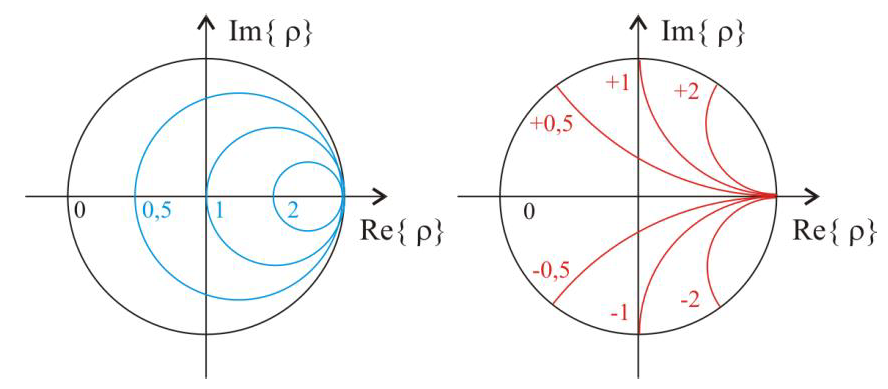
\includegraphics[scale=0.5]{ANT/kruznice_konstanteho_normovaneho_odporu_reaktancie.png}}
	\captionsetup{justification=centering}
	\caption{Kružnice konštantného normovaného odporu (vľavo), kružnice konštantnej normovanej reaktancie (vpravo)}
	\label{fig:smith}
\end{figure}
Postup:
\begin{itemize}[label = ]
\item 1. Normujeme impedanciu záťaže $z = Z/Z_V$ a vynesieme ju do diagramu 
\item 2. Odčítame zodpovedajúci činiteľ odrazu $\rho$
\item 3. Otočíme fázor o $l/\lambda$ jednotiek v smere ku zdroju (alebo k záťaži)
\item 4. Pre stratové vedenie, vynásobíme modul činiteľa odrazu činiteľom $\exp(-2\beta l)$
\item 5. Odčítame normovanú vstupnú impedanciu a vynásobíme $Z_V$
\end{itemize}

\subsection{Vedenia a zakončenia vedení}

\textbf{Štvrťvlnné vedenie} ($l = \lambda/4$) -- vstupná impedancia je nepriamo úmerná záťažovej $Z(l) = Z_V^2/Z(0)$. Reálna záťaž zostáva na vstupe reálna.\\
\medskip
\textbf{Polvlnné vedenie} ($l = \lambda/2$) -- na vstupe namerané presne zaťažovaciu impedanciu $Z(l) = Z(0)$\\
\medskip

\textbf{Prispôsobené vedenie} ($Z(0) = Z_V$)  -- kdekoľvek na vedení je impedancia rovnaká a rovná sa charakteristickej. Nenastáva žiadný odraz, v Smithovodm diagrame leží v strede ($\rho$ = 0)\\
\medskip

\textbf{Vedenie nakrátko} ($Z(0) = 0$) -- Na vstupe nameráme čistú reaktanciu, ktorá mení charakter podľa dĺžky -- pre $l < \lambda/4$ je induktívna, pri $l = \lambda/4$ nastáva paralelná rezonancia, pre $\lambda/4 < l < \lambda/2$ je kapacitná a pri $l \approx \lambda/2$ nastáva sériová rezonancia. Pre $l > \lambda/2$ sa priebeh opakuje.\\
\medskip

\textbf{Vedenie nakrátko} ($Z(0) \rightarrow \infty$) -- Správa sa rovnako ako vedenie nakrátko, ale celý priebeh reaktancie je posunutý o $\lambda/4$ - pre $l < \lambda/4$ má kapacitný charakter a nasleduje sériová rezonancia.\\
\medskip

\begin{figure}[H]
	%\vspace{-2mm}
	\makebox[\textwidth]{%
		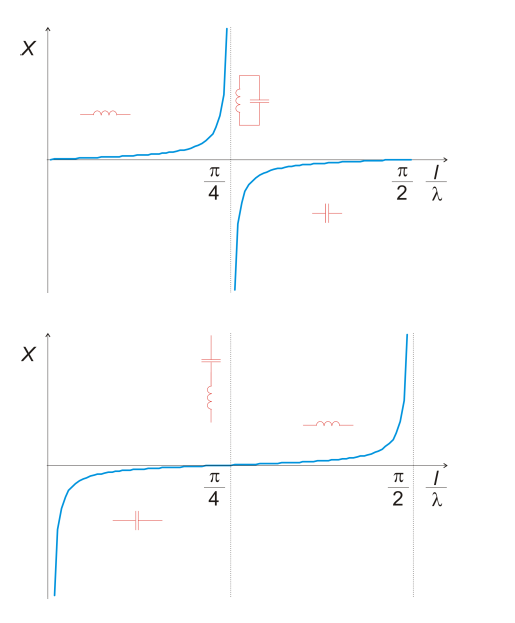
\includegraphics[scale=0.5]{ANT/reaktancia_useky.png}}
		\captionsetup{justification=centering}
	\caption{Reaktancia na vstupe úseku vedenia na konci nakrátko (hore)
		a na konci naprázdno (dole).}
	\label{fig:useky_reaktancia}
\end{figure}

\newpage
\subsection{Impedančné prispôsobenie}

Vedenie optimálne prenáša elektromagnetickú energiu, ak sa záťažová impedancia rovná charakteristickej impedancii ($Z_k = Z_V$). Pri splnení tejto podmienky platí:
\begin{itemize}[label =--]
%\vspace*{-2mm}
\item Po vedení sa šíri iba priama vlna
\item Účinnosť prenosu energie je najväčšia
\item Vstupná impedancia vedenia je reálna a stála
\item Napätia a prúdy na vedení sú pri danom prenášanom výkone najmenšie
\end{itemize}

Ak záťaž podmienku nespĺňa ($Z_k \neq Z_V$), je nutné medzi vedenie a záťaž zapojiť prispôsobovací obvod, ktorý transformuje $Z_k$ na hodnotu $Z_V$.
Ideálne podmienky (PSV = 1, $\rho$ = 0), ak to nie je možné dosiahnuť podľa kvality sa rozoznáva: 
\begin{itemize}[label = $\square$]
%\vspace*{-2mm}
\item veľmi dobré prispôsobenie je PSV < 1,1 (napr. televízne vysielače) 
\item dobré prispôsobenie PSV < 1,5 až 2,0 (bežné zariadenia)
\item vyhovovujúce prispôsobenie PSV < 3,0 až 5,0 (nenáročne zariadenia)
\end{itemize}

\textbf{Metódy prispôsobenia:}\\
\medskip
\textbf{Vloženie vedenia}\\
Medzi záťaž a napájacie vedenie sa vloží úsek vedenia s charakteristickou impedanciou $Z_T$ a dĺžkou $l_T$. Metóda je jednoduchá, ale obmedzená (nedá sa transformovať ľubovoľná impedancia), platí, že:
			
\begin{equation}
	\frac{Z_V}{R_k} \geq 1 + \left(\frac{X_k}{R_k}\right)^2,
	\qquad
	\frac{Z_V}{R_k} \leq 1
\end{equation}


\textbf{Štvrťvlnný transformátor}\\
Spočíva vo vložení prenosového vedenia (s dĺžkou $l = \lambda/4$) do série medzi napájacie vedenie (zdroj) a záťaž 

\begin{figure}[H]
	%\vspace{-2mm}
	\makebox[\textwidth]{%
		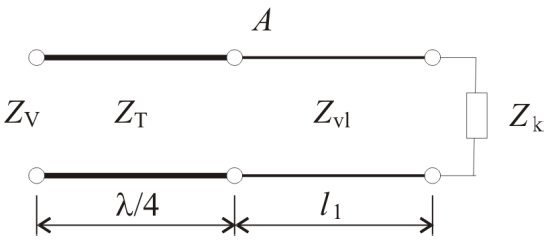
\includegraphics[scale=0.5]{ANT/stvrtvlnne_vedenie_transf.png}}
	\captionsetup{justification=centering}
	\caption{Prispôsobenie vloženým vedením a štvrťvlnným transformátorom}
	\label{fig:stvrtvlnne_transf}
\end{figure}

Aby došlo k dokonalému prispôsobeniu musí platiť:
\begin{equation}
	Z_{OT} = \sqrt{Z_{OV} Z_{K}}
\end{equation}

-- Štvrťvlnný transformátor je použiteľný iba pre reálne záťaže\\
-- Z kmitočtového hľadiska je úzkopásmovy\\
\bigskip
Často sa používa kombinácia vloženého vedenia (s dĺžkou $l_1$) a štvrťvlnného transformátora, ktorá je zobrazená na obr. \ref{fig:stvrtvlnne_transf}.\\\medskip
\textbf{Vložené vedenie} (dĺžka $l1$) -- transformuje komplexnú impedanciu záťaže $\rightarrow$ zostane iba reálna zložka \\
\textbf{Štvrťvlnný transformátor} ($l=\lambda/4$) -- transformuje reálne hodnoty na požadovanú reálnu impedanciu napájacieho vedenia $Z_{V}$

\newpage
\textbf{Sériový pahýľ}\\
Spočíva v návrhu dĺžky vloženého vedenia, kde sa reálna zložka impedancie rovná charakteristickej impedancii napájacieho vedenia ($R_1 = Z_V$). \\
-- vloženie pahýľa do tohto miesta vykompenzuje stále prítomnú imaginárnu zložku reaktanciou pahýľu $X_{pahyl} = -X_1$ 

\begin{figure}[H]
	%\vspace{-2mm}
	\makebox[\textwidth]{%
		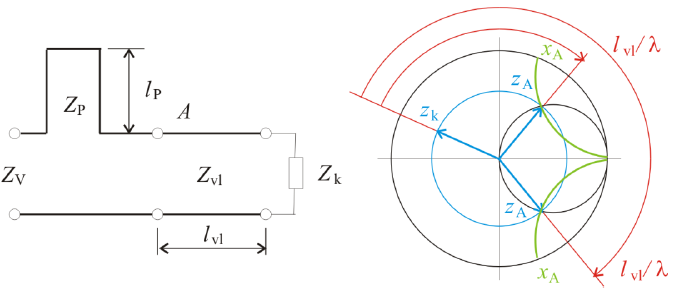
\includegraphics[scale=0.5]{ANT/seriovy_pahyl.png}}
	\captionsetup{justification=centering}
	\caption{Prispôsobenie pomocou sériového pahýľa}
	\label{fig:seriovy_pahyl}
\end{figure}

\textbf{Paralelný pahýľ}\\
Vychádza z odstránenia nevýhody rozpojenia vedenia pri riešení so sériovým pahýľom. Spočíva v návrhu dĺžky vloženého vedenia, kde sa reálna zložka admitanice (vodivosti G) rovná charakteristickej admitancii napájacieho vedenia ($Y_V = \frac{1}{Z_V}$)\\
-- vloženie paralelného pahýľa do tohto miesta vykompenzuje stále prítomnú imaginárnu zložku admitancie susceptanciou pahýľa $B_{pahyl} = - B_1$
\begin{figure}[H]
	%\vspace{-2mm}
	\makebox[\textwidth]{%
		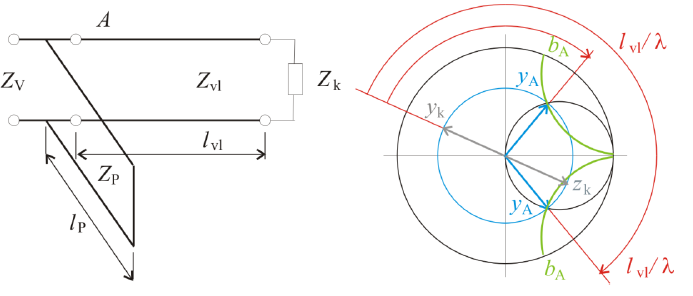
\includegraphics[scale=0.5]{ANT/paralelny_pahyl.png}}
	\captionsetup{justification=centering}
	\caption{Prispôsobenie pomocou paralelného pahýľa}
	\label{fig:paralelny_pahyl}
\end{figure}

\newpage
\chapter{Antény, Dipólové a flíčkové antény.}

\textbf{PRE 3. OTÁZKU JE NAJLEPŠIE SI PREČÍTAŤ DOKUMENT BEVA\_08 A BEVA\_10, NIŽŠIE JE IBA KRÁTKE ZHRNUTIE}

\subsection{Antény}
Anténa je transformačný prvok, ktorý prevádza elektromagnetickú vlnu šíriacu sa pozdĺž vedenia na vlnu voľným priestorom. Vychádza sa z dvojvodičového vedenia zakončeného naprázdno -- otočením koncov o 90$\degree$ vznikne symetricky napájaný dipól.

\begin{figure}[H]
	%\vspace{-2mm}
		\makebox[\textwidth]{%
			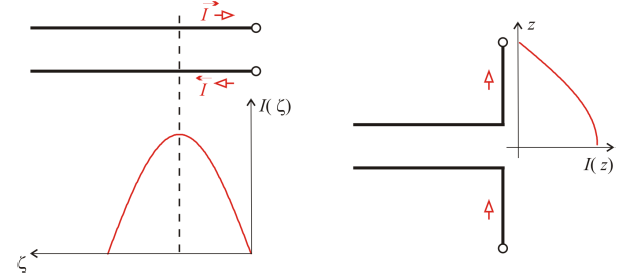
\includegraphics[scale=0.45]{ANT/anteny.png}}
		\captionsetup{justification=centering}
		\caption{Dvojvodičové vedenie na konci naprázdno (vľavo), symetricky budený polvlnný dipól (vpravo)}
	\label{fig:anteny_dipol}
\end{figure}

Oboma ramenami dipólu pretekajú prúdy so súhlasnou orientáciou, v okolí vodiča vzniká podľa Ampérová zákona axiálne magnetické pole. Vlna šíriaca se od dipólu v radiálnom smere bude mať v dostatočnej vzdialenosti elektrickú zložku poľa, ktorá je kolmá jak na smer šírenia, tak na zložku magnetickú.

\begin{figure}[H]
	%\vspace{-2mm}
	\makebox[\textwidth]{%
		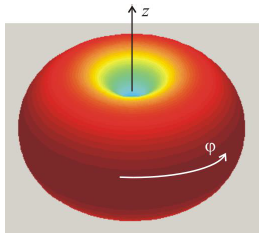
\includegraphics[scale=0.45]{ANT/vyzarovanie_sym_dipolu.png}}
	\captionsetup{justification=centering}
	\caption{Vyžarovanie symetrického dipólu rovnobežného s osou $z$}
	\label{fig:symetricky_dipol_vyzarovanie}
\end{figure}
 Dipól nevyžaruje do smeru svojej osy, maximum vyžarovania je kolmé na osu dipólu.

\subsection{Ekvivalentný obvod}
\underline{Rezistor $R_{ztr}$} -- vyjadruje straty v anténe, dané nedokonalou vodivosťou anténneho vodiča (elektromagnetická energia sa mení na energiu tepelnú, kov sa zahrieva). \\
\underline{Rezistor $R_{\Sigma}$} -- reprezentuje premenu elektromagnetickej energie dodávanej do antény na energiu vyžarovanú.\\
\underline{Reaktancia $X_{\Sigma}$} -- reprezentuje prelievanie jalového výkonu z antény do iného blízkeho poľa a späť (obdoba prelievania energie do magnetického poľa cievky).

\begin{figure}[H]
	%\vspace{-2mm}
	\makebox[\textwidth]{%
		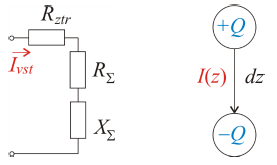
\includegraphics[scale=0.65]{ANT/ekvivalentny_obvod_anteny.png}}
	\captionsetup{justification=centering}
	\caption{Ekvivalentný obvod antény (vľavo). Elementárny dipól (vpravo).}
	\label{fig:ekvivalentny_obvod_anteny}
\end{figure}
Činný výkon vyžarovania antény:
\begin{equation}
	P_{\Sigma} = R_{\Sigma,m} I_m^2
\end{equation}

\subsection{Vstupná impedancia}
Vstupná impedancia antény, ktorú pozorujeme na svorkách je rovná súčtu:
\begin{equation}
	Z_{vst} = R_{\Sigma vst} + R_{ztr} + jX_{\Sigma vst}
\end{equation}


\subsection{Elementárny žiarič}
Elementárny dipól je nekonečne krátky úsek drôtového dipólu, na ktorom možno predpokladať konštantný prúd $I$. Používa sa pre zjednodušenie matematického popisu antén. \\
\medskip
Príspevok náboja v pohybu (príspevok prúdu) k vyžarovaniu vlny popisujeme vektorovým potenciálom:\\
%\vspace*{-1mm}
\begin{equation}
	dA_z(z') = \frac{\mu_0}{4\pi} I(z) dz \frac{\exp(-jkr)}{r}
\end{equation}

Intenzitu elektrického poľa antény je možné vyjadriť vzťahom:
\begin{equation}
	E = 60 I F(\varphi,\vartheta)  \frac{\exp(-jkr)}{r}
\end{equation}

\subsection{Smerová charakteristika}

Smerová charakteristika je grafickým znázornením absolútnej hodnoty pomernej (normovanej) funkcie žiarenia $F/F_{max}$. Vynáša sa v polárnych nebo kartézských súradniciach.\\
\medskip
Funkcia žiarenia elementárneho dipólu je:
\begin{equation}
	F(\varphi,\vartheta) = j \frac{k}{2} \sin\vartheta dz
\end{equation}
Funkcia žiarenia popisuje smerové vlastnosti antény. Rôzne antény sa líšia funkciou $F$. Vzhľadom k súradnici $\varphi$ žiari dipol do všetkých smerov. 

\begin{figure}[H]
	%\vspace{-2mm}
	\makebox[\textwidth]{%
		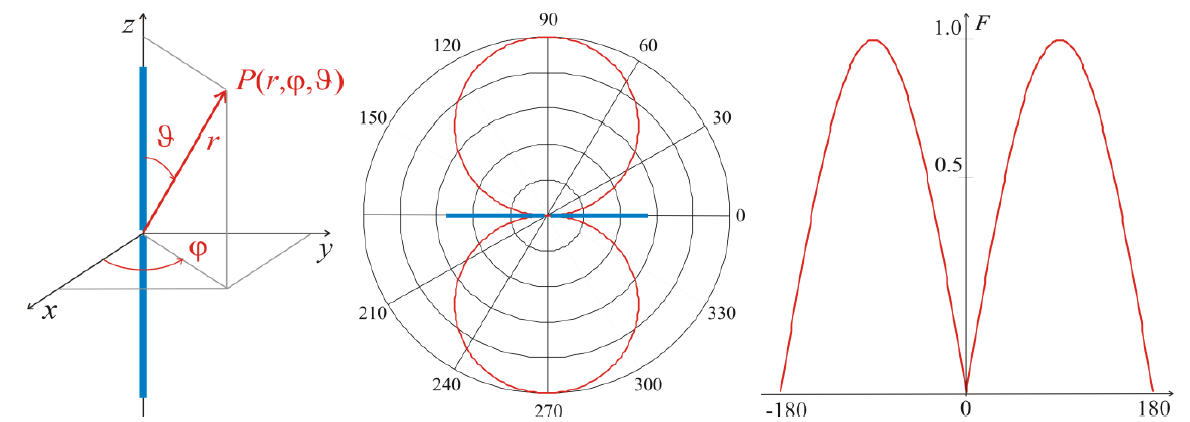
\includegraphics[scale=0.4]{ANT/elementarny_dipol_charakteristiky.png}}
	\captionsetup{justification=centering}
	\caption{Elementárny dipól (vľavo). Smerová charakteristika elementárneho dipólu v polárnych súradniciach (uprostred) a kartézských súradniciach (vpravo)}
	\label{fig:elementarny_dipol_charakteristiky}
\end{figure}

Pomer veľkosti funkcie žiarenia v danom smere $F(\varphi,\vartheta)$ k maximu žiarenia $F_{max}$ vyjadruje smerovú závislosť vyžarovania a nazýva sa \textit{pomerná (normovaná)} funkcia žiarenia. Pre elementárny dipól $F/F_{max} = \sin \vartheta$.

\subsection{Technický výpočet žiarenia anténnych sústav}

Anténa sústavu tvorí skupina anténnych prvkov, napájaných zo spoločného zdroja. Hlavným dôvodom je zoskupenie antén do sústav je ľahšie dosiahnutie požadovaných smerových vlastností. \\ \bigskip Vlastnosti anténnych sústav sú určené usporiadaním prvkov v priestore, vlastnosťami každého prvku a amplitúdami a fázami prúdu v prvkoch.
\medskip
\begin{figure}[H]
	%\vspace{-2mm}
	\makebox[\textwidth]{%
		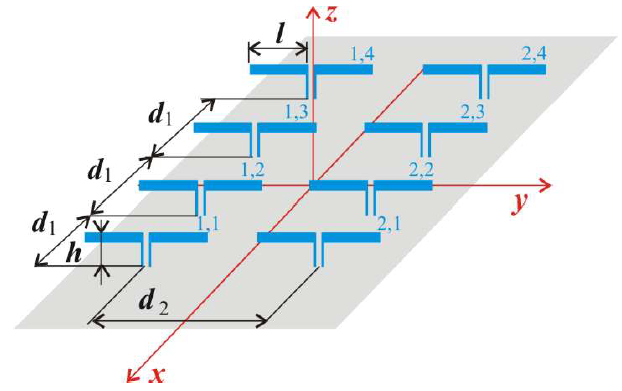
\includegraphics[scale=0.4]{ANT/zadanie_projekt.png}}
	\captionsetup{justification=centering}
		\caption{Sústava dipólov}
	\label{fig:zadanie_projekt}
\end{figure}

Pri výpočte žiarenia anténnej sústavy sa sčítajú príspevky jednotlivých prvkov vo vzdialenom bode (trajektórie vĺn sú paralelné). Prúdy v prvkov aj prvky sústavy sú rovnaké (každý prvok je popísaní funkciami žiarenia).\\
 \bigskip
Výsledná funkcia žiarenia je rovná súčinu funkcii žiarenia prvkov -- princíp násobenia charakteristík. 

\begin{figure}[H]
	%\vspace{-2mm}
	\makebox[\textwidth]{%
		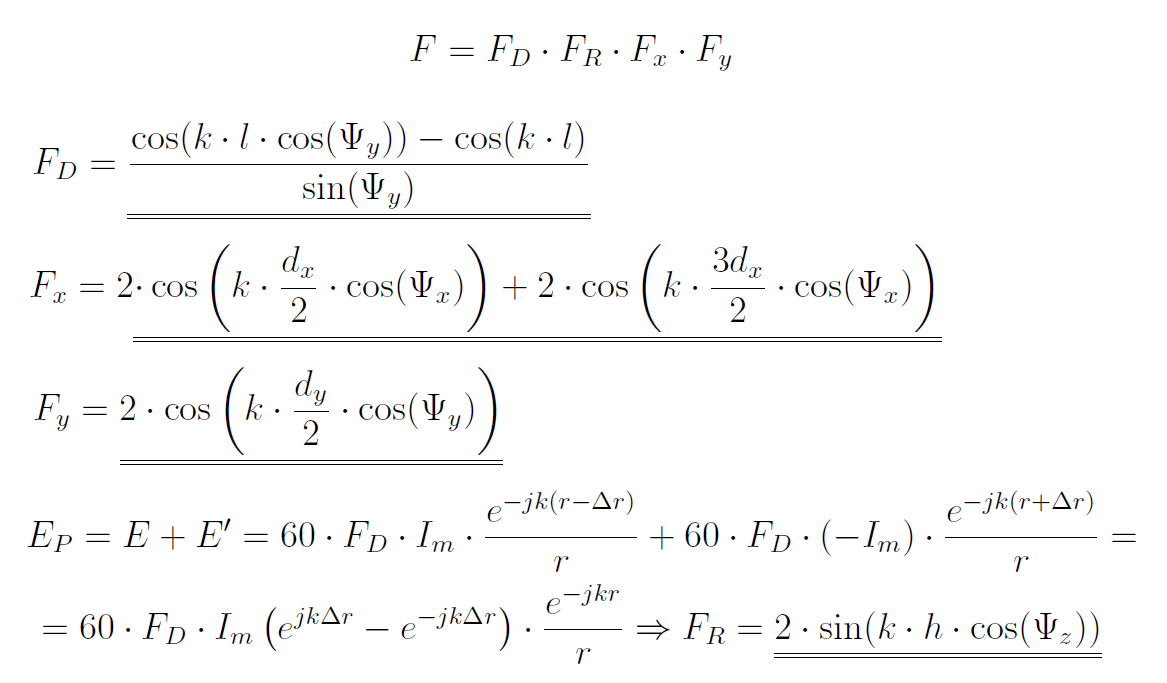
\includegraphics[scale=0.4]{ANT/vypocet_vyzarovacej_funkcie.png}}
	\captionsetup{justification=centering}
	\caption{Výpočet vyžarovacej funkcie}
	\label{fig:vypocet_vyzar_funkcie}
\end{figure}

\newpage
\subsection{Smerovosť}

Smerovosť je udávaná činiteľom smerovosti $D(\varphi, \vartheta)$, ktorý popisuje, do ktorých smerov vyžaruje anténa väčší výkon a do ktorých výkon menší. Činiteľ smerovosti $D$ zároveň dovoľuje vypočítať intenzitu poľa $E$, ak poznáme vyžarovaný výkon. 

\begin{equation}
	E = \frac{\sqrt{30 P_{\Sigma} D(\varphi,\vartheta)}}{r}
\end{equation}

Výpočet činiteľa smerovosti:
\begin{equation}
	D(\varphi, \vartheta) = \frac{120}{R_{\Sigma m}} \abs{F(\varphi,\vartheta)}^2
\end{equation}

kde $R_{\Sigma m}$ je odpor žiarenia vztiahnutý ku kmitne.\\\medskip
Činiteľ smerovosti závisí iba na tvare smerovej charakteristiky. Pre anténu s dobre vyjadreným lalokom doutníkového tvaru platí približný vzťah:

\begin{equation}
	D_{max} = \frac{35000}{2\theta_E 2\theta_H}
\end{equation}
kde $2\theta_E $ a $2\theta_H$ sú uhlové (celé) šírky hlavného laloka ve dvoch navzájom kolmých
rovinách (v rovinách E a H), vyjadrené vo stupňoch.

\subsection{Zisk}
Zisk antény je definovaný ako súčin činiteľa smerovosti vo smere maxima žiarenia a účinnosti antény. Zisk sa vyjadruje v decibeloch:
\begin{equation}
	G = 10 \log(\eta D_{max})
\end{equation}

\subsection{Polarizácia}

Polarizácia antény je vlastnosť, ktorá popisuje smer kmitania elektrického poľa vyžiarenej elektromagnetickej vlny. Tento smer je vždy zhodný s osou dipólu. \\
\medskip
Podľa orientácie dipólu rozlišujeme vertikálnu a horizontálnu polarizáciu. Pri vertikálnej polarizácii je dipól postavený zvisle, pri horizontálnej leží vodorovne. Okrem týchto dvoch základných typov existuje aj kruhová polarizácia, kde sa smer elektrického poľa závitovo otáča pozdĺž smeru šírenia vlny.

\newpage
\subsection{Dipólové antény}

Dipólová anténa je lineárna anténa, kde zdrojom žiarenia je priamy vodič pretékaný vysokofrekvenčným prúdom. Vzniká z otvoreného dvojvodičového vedenia otočením koncov o 90\degree.\\
\bigskip
\textbf{Druhy}:\\
\underline{Polvlnný dipól} má celkovú dĺžku $\lambda/2$, každé rameno $\lambda/4$. Je to najpoužívanejší typ. \\
\underline{Monopól} je jedno rameno dipólu nad vodivou plochou — správa sa ako celý dipól, ale vyžaruje len do horného polopriestoru. \\
\bigskip
\textbf{Smerové vlastnosti:}
Dipól nevyžaruje do smeru svojej osi, maximum je kolmé na os. Pri predlžovaní ramena sa žiarenie koncentruje kolmo na os, pri prekročení $\lambda/2$ vznikajú bočné laloky. Smerové vlastnosti sústavy možno ďalej meniť fázovaním budiacich prúdov. Rovinný reflektor umiestnený za dipólmi potlačí žiarenie dozadu a zdvojnásobí efektívne žiarenie dopredu.
\medskip
\begin{figure}[H]
	%\vspace{-2mm}
	\makebox[\textwidth]{%
		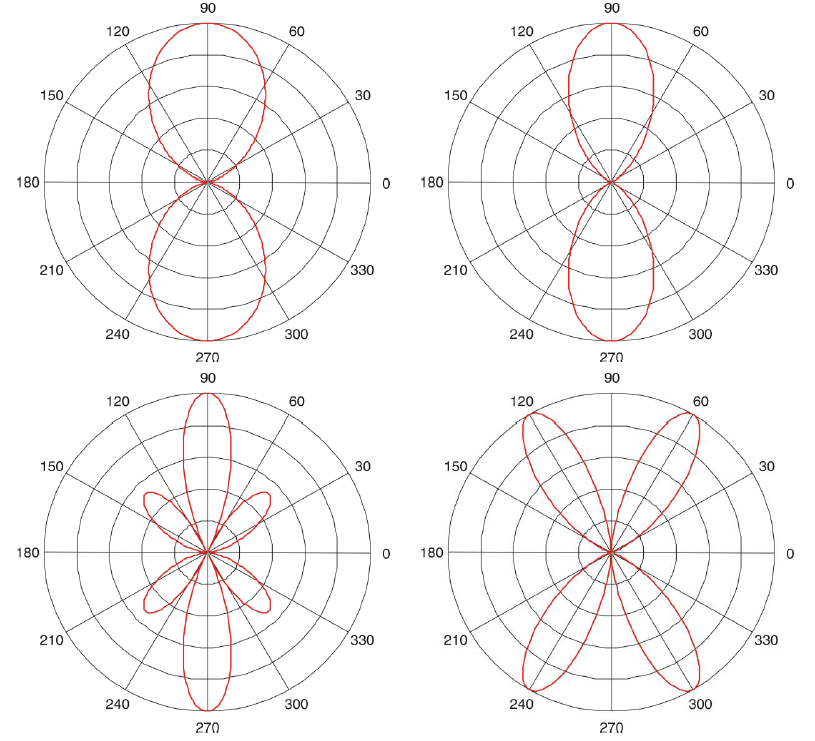
\includegraphics[scale=0.5]{ANT/smerove_char_sym_dipolov.png}}
	\captionsetup{justification=centering}
	\caption{Smerové charakteristiky symetrického dipólu:\\ $l/\lambda$ = 0,25 (vľavo hore), $l/\lambda$ = 0,5 (vpravo hore)\\ $l/\lambda$ = 0,7 (vľavo dole), $l/\lambda$ = 1 (vpravo hore) }
	\label{fig:smerove_char_sym_dipolov}
\end{figure}
\bigskip
\textbf{Anténne sústavy:}
Dipóly možno združovať do sústav. Výsledná funkcia žiarenia je súčinom funkcie žiarenia prvku a skupinovej funkcie -- princíp násobenia charakteristík. Hlavné parametre každej antény sú činiteľ smerovosti $D$, účinnosť $\eta$, zisk $G$ a účinná dĺžka.



\newpage
\subsection{Flíčkové antény}

Flíčková anténa je najjednoduchší typ plošnej antény, kde zdrojom žiarenia nie je lineárny vodič, ale plocha rozložená v dvoch rozmeroch. Skladá sa z kovového flíčka umiestneného na dielektrickom substráte nad zemnou plochou.\\
\bigskip
\textbf{Napájanie}:\\
\underline{Mikropáskové vedenie} -- jednoduchá výroba, ale parazitné vyžarovanie deformuje smerovú charakteristiku.\\ 
\underline{Koaxiálna sonda} -- bez parazitného vyžarovania, ale náročnejšia výroba (vŕtanie do substrátu)\\
\medskip

\textbf{Smerové vlastnosti:}\\
Vyžarujú prednostne kolmo na rovinu flíčka, teda hlavný lalok smeruje kolmo od substrátu. V smere roviny substrátu je vyžarovanie minimálne. Smerová charakteristika je relatívne široká.\\ 
\medskip
Konkrétny tvar charakteristiky závisí od rozmerov flíčka, vlastností substrátu a spôsobu napájania. Parazitné vyžarovanie napájacieho mikropásku môže charakteristiku deformovať, čo je jedna z nevýhod mikropáskového napájania oproti koaxiálnej sonde.\\
\bigskip
\textbf{Návrh}:\\
Potrebujeme poznať výšku substrátu $h$, permitivitu $\varepsilon_r$ a činiteľ strát $\tan \delta$. Postup: vypočítame vlnovú dĺžku $\rightarrow$ šírku flíčka $W$ $\rightarrow$ efektívnu permitivitu $\varepsilon_{ef}$ $\rightarrow$ dĺžku flíčka $L = \lambda/2$.\\
\medskip
\textbf{Impedančné prispôsobenie}\\
Napätie na flíčku klesá od hrán k stredu, zatiaľ čo prúd rastie od hrán k stredu. Poloha napájacieho bodu priamo určuje vstupnú impedanciu: čím bližšie k stredu, tým nižšia impedancia. Na mikrovlnných kmitočtoch sa štandardne pracuje s impedanciou 50 $\Omega$.\\
\medskip
\textbf{Dvojpásmová prevádzka}\\
Dvojpásmového správania možno dosiahnuť vyleptaním dvojice štrbín do anténneho prvku. Na nižšom kmitočte sa prúdová polvlna rozloží cez celý flíček, na vyššom kmitočte iba cez oblasť ohraničenú štrbinami.



%\end{document}



 